\section{Coding}\label{sec:coding}

The central part of a genetic approach to the painting placement problem is how an individual is represented.
This is important not only for the construction of the genetic operators, e.g., crossover and mutation but also for the process of decoding an individual from its representation to the solution.


In this thesis, an individual is represented as a 3D—which means having three genes—chromosome that is composed of
(1) painting sequence random key, (2) slicing order random key, and (3) orientation probabilities.
An example of chromosome is in figure~\ref{fig:chromosome}

Let us use the notation for painting sequence random key as $PS_{rk}$,
slicing order random key as $SO_{rk}$,
orientation probabilities as $OR_{prob}$ and instance size as $N$, i.e., number of paintings.
First two are vectors, where $PS_{rk} \in \real^N$ and $SO_{rk} \in \real^{N-1}$.
Orientation probabilities is a matrix where $OR_{prob} \in \real^{N-1, N-1}$.

Multiple constraints apply to each part of a chromosome.

\begin{itemize}
    \item Painting sequence random key is a stochastic vector.
    \item Slicing order random key is a stochastic vector.
    \item Each row in orientation probabilities is a stochastic vector.
\end{itemize}

Here, a stochastic vector means a vector that contains non-negative elements that add up to one.
The reasoning behind the decision to represent an individual in this way is given later in the text.

The above-mentioned representation is based on a solution to the facility layout problem using a slicing tree representation
from~\cite{friedrichIntegratedSlicingTree2018},
where the author also represents an individual as a 3D chromosome.
However, the difference is that in this thesis, each part is a stochastic vector while
in~\cite{friedrichIntegratedSlicingTree2018} author uses concrete identifiers of facilities, slicing order, and orientation.
Thus, in this thesis, an additional decoding layer is introduced together with different genetic operators.

\begin{figure}[htp]
    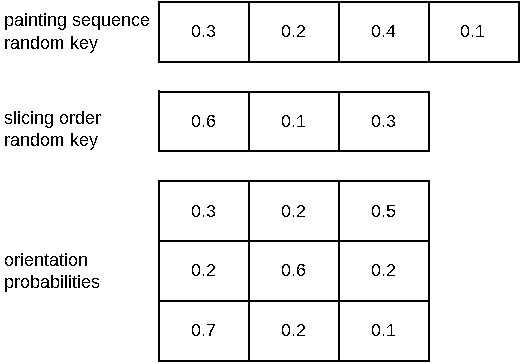
\includegraphics[width=0.8\textwidth, center]{chromosome}\caption[Example of an individual representation]{
        Example of an individual representation – two vectors and one matrix.
        Each vector and matrix row form a stochastic vector, i.e., they contain non-negative elements that add up to 1.
    }
    \label{fig:chromosome}
\end{figure}
